\chapter{System Design and Methodology}\label{ch:design}
\section{Proposed System Architecture}
Figure~\ref{fig:architecture} shows the inference path. The system boundary is a web application: photographs come in through the browser, the stage, the driving photograph and the PDF go out. Inside, four stages are chained: fundus preprocessing, a per-photograph classifier, the worst-view aggregation rule, and the report generator. The classifier is swappable by configuration; the rest of the pipeline is model-independent, which is what allowed nine models to be compared without touching the application.
\begin{figure}[htbp]
\centering
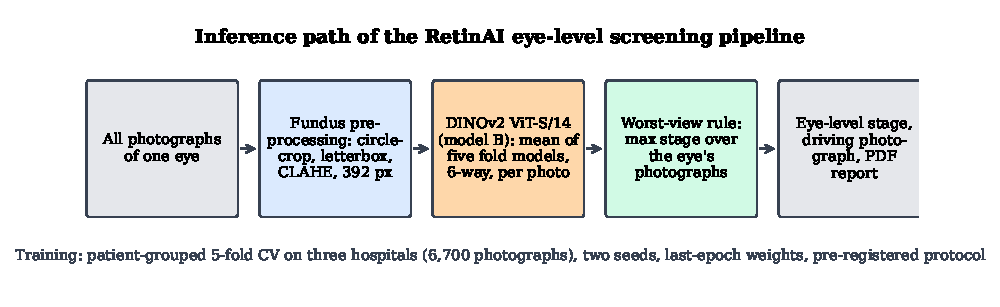
\includegraphics[width=\textwidth]{fig_pipeline.pdf}
\caption{RetinAI system architecture: the inference path from the photographs of one eye to its stage}\label{fig:architecture}
\end{figure}

\textbf{Preprocessing.} Each photograph is circle-cropped to the fundus, padded to a square (letterbox), contrast-enhanced with CLAHE, and resized to 392~px. For training, this stage runs once per image and the result is cached at 768~px, so that each Kaggle session reads pre-processed files rather than repeating the work 20 times.

\textbf{Per-photograph classifier.} A vision transformer, ViT-S/14 with four register tokens (21.8~M parameters, 12 layers, width 384, 6 heads), takes the 392~px photograph as 784 patches, averages the patch outputs, and passes them through dropout (0.3) and a linear layer with six outputs: normal, stage~1, stage~2, stage~3, stage~4/5 and AP-ROP. The same head sits on the EfficientNetV2-S baseline. In the application the selected model~B is served as the mean of the probabilities of its five cross-validation fold models (seed 42), so that no single fold's validation infants are missing from what the served model has learnt.

\textbf{Worst-view rule.} The eye's stage is the maximum predicted stage over its photographs; the photograph that attains it is the driving photograph, and its probability vector is the eye's probability vector. This is the reading rule of ICROP: an eye is staged by its most advanced finding.

\textbf{Report.} The eye summary, the per-photograph table and the driving photograph are rendered into a PDF.

\section{Design Alternatives and Selection}
Three families of design were considered for the eye-level requirement and the "different model" requirement.

\textbf{Learned aggregation versus the worst-view rule.} A gated-attention multiple-instance model that learns how to combine the photographs of an eye was built and tested on frozen features before the main design. It tied the worst-view rule in cross-validation ($-0.006$ QWK) and lost on the held-out hospital's eyes ($-0.080$ QWK, interval excluding zero), because the only multi-photograph training bags are mostly normal Ostrava sessions, so the learned combiner under-calls disease. The worst-view rule was selected: it needs no eye-level training data, it is the clinical rule, and it is explainable (the driving photograph is shown).

\textbf{Backbone.} The candidates were a retina-pretrained transformer (RETFound-Green), a natural-image-pretrained transformer of identical architecture (DINOv2 ViT-S/14), larger transformers (RETFound ViT-L, DINOv2 ViT-B), and classical CNNs (VGG, ResNet). A frozen-feature spike showed RETFound-Green with CLAHE as the best frozen encoder (0.859 CV QWK against 0.796 for frozen ImageNet EfficientNet) but behind the fine-tuned EfficientNet (0.917), so the lever is fine-tuning, not the encoder alone. Paper~1 had already shown five backbones within 0.028 macro-F1 of one another. The ViT-S pair was selected because it isolates the one variable not yet tested in the literature, the pre-training domain, with every other factor equal; larger models were rejected on Kaggle's time limits and because the question is about domain, not size; VGG and ResNet were rejected as older designs that paper~1's benchmark had already placed in the same band.

\textbf{Training unit.} For the Ostrava cohort, whose labels are per examination session, two options exist: per-image cross-entropy against the stamped label (the baseline) or a per-session loss that pools the frames. Log-sum-exp pooling of the frames' logits with $K=8$ frames per session was selected over mean or attention pooling, because it trains all frames while letting the most abnormal frame dominate, which matches how the session label was produced.

\section{Software and Algorithm Design}
Figure~\ref{fig:architecture} is implemented as five modules: \texttt{preprocessing} (transforms, cache, normalisation per arm), \texttt{architectures} (backbone construction, strict loading of RETFound-Green weights), \texttt{optim} (per-layer learning-rate groups), \texttt{train\_utils} (training loop, bag loss, adaptation), and \texttt{inference} (eye-level route). The experiment side consists of the Kaggle kernel, a pusher that rewrites the kernel's knobs, a collector that validates downloaded runs, and a scorer that computes every protocol metric from saved predictions. The eye-level inference algorithm is:
\begin{enumerate}
\item for each photograph $i$ of the eye, compute the probability vector $\mathbf{p}_i\in\mathbb{R}^6$ and the predicted class $\hat{y}_i=\arg\max_c p_{i,c}$;
\item the eye's stage is $\hat{y}=\max_i \hat{y}_i$ on the ordered stage axis, with AP-ROP reported when it is any photograph's argmax;
\item the driving photograph is $i^\star=\arg\max_i(\hat{y}_i, p_{i,\hat{y}_i})$, ties broken by its probability, and the eye's probability vector is $\mathbf{p}_{i^\star}$;
\item the any-ROP score of the eye is $\max_i(1-p_{i,\text{normal}})$, compared with the pre-registered threshold.
\end{enumerate}

\section{Mathematical Model and Design Calculations}
\textbf{Loss.} Each arm minimises class-balanced cross-entropy with label smoothing. With $n_c$ training images of class $c$ and $\beta=0.999$, the class weight is the inverse effective number of samples,
\begin{equation}\label{eq:cb}
w_c=\frac{1-\beta}{1-\beta^{\,n_c}},\qquad
\mathcal{L}=-\sum_{c}w_c\,\tilde{y}_c\log p_c,
\end{equation}
where $\tilde{y}$ is the one-hot label smoothed by $\varepsilon=0.05$. Rare stages (89 stage-4/5 images against 3{,}837 normal) therefore count more per image.

\textbf{Examination-level loss (model D).} For an Ostrava session with frames $1..K$ and per-frame logits $\mathbf{z}_k$, the session logit is the log-sum-exp pool
\begin{equation}\label{eq:lse}
\mathbf{z}_{\text{session}}=\tau\log\sum_{k=1}^{K}\exp(\mathbf{z}_k/\tau),\qquad \tau=1,
\end{equation}
and Equation~\ref{eq:cb} is applied to it with the session's label. A one-frame session reduces exactly to per-image cross-entropy.

\textbf{Optimiser.} AdamW with weight decay 0.05, a one-cycle cosine schedule with 10\% warm-up, and layer-wise decay: layer $\ell$ of the 12 transformer layers trains at $\eta\,\lambda^{13-\ell}$ with $\lambda=0.8$, so the patch embedding trains at $0.8^{13}\eta\approx0.055\eta$ and the head at $\eta$. The peak $\eta$ was chosen per arm by a probe on an inner split of fold~0 (never on fold~0's validation rows): $2\times10^{-4}$ for RETFound-Green and $10^{-4}$ for DINOv2, keeping the default unless a candidate beat it by more than 0.03 macro-F1.

\textbf{Compute budget.} At 30 photographs/s, one fold of 2{,}460 training images for 20 epochs takes $2{,}460\times20/30\approx1{,}640$~s of training plus validation and dev scoring, about 33~min measured; five folds and the site fold fit one 8~h kernel with margin (3.3~h measured). At 518~px the cost is $(518/392)^4\approx3.0\times$ in attention and 2.3$\times$ measured, so model~G was split over two kernels. In the v4 round each model and seed also ran two LOSO folds, of which the Ostrava fold alone takes about 50~min, so H and I used two kernels per seed (five cross-validation folds; site fold and two LOSO folds).

\textbf{Statistics.} All intervals are percentile bootstrap intervals over 2{,}000 resamples of infants (eyes of one infant kept together). A paired difference between two arms is computed on the same resample. The minimum detectable eye-level QWK difference at 80\% power on the 230-eye locked half is about 0.08, which was stated in the protocol before any model was trained.

\section{The v4 Round: Data Audit, Training Pool and Recipe}\label{sec:v4design}
After the seven models of the v3 round had been scored, the protocol's fifth amendment (31 October 2026, before any v4 run or locked scoring) fixed one final improvement round on the selected model~B. Models A--G were frozen. Two levers were left untested by v3: the training data of the video-derived Ostrava cohort, and the training recipe. The round tests each separately: model~H is B's recipe on a cleaned training pool, and model~I adds a regularising recipe on the same pool. Validation rows, folds and the duplicate exclusion are unchanged, so every model is scored on the same 6{,}686 photographs.

\textbf{Frame quality, judged per camera.} Ostrava's frames come from three camera models whose sharpness and exposure differ systematically. The first design took its thresholds from the two single-photograph hospitals (ROP-VL and Shenzhen, whose photographs were already selected by clinicians), including a minimum field of view. The audit rejected it before the pool was built: the field-of-view minimum is a property of the camera's aperture, and it failed 903 of the 911 frames of one camera, among them all 125 Ostrava stage-3 frames. The selected design judges each frame against its own camera: a frame fails if it is empty, if its sharpness (variance of the Laplacian) is below its camera's 10th percentile, or if its mean luminance is outside its camera's 2.5th--97.5th percentiles. ROP-VL and Shenzhen are not filtered, because their haze is often the disease.

\textbf{Cap re-ranking and floor.} The per-infant caps are unchanged (two normal frames, twenty frames per stage), but within each infant and class the kept frames are the passing frames with the highest sharpness rank, instead of the first by file name; an infant and class with fewer than two passing frames keeps its two best, so no infant loses a class.

\textbf{Near-duplicates.} Every pair of pool photographs at a 256-bit difference-hash (dHash) distance of at most 4 was checked by the mean absolute grey-level difference of the two images at 256$\times$256 pixels; both members of a cross-fold pair with a difference of at most 5 grey levels leave the training rows. The hash alone was rejected, because it matched distinct Ostrava retinas (9--47 grey levels apart) as well as true copies (about 3 grey levels apart within a session). Pairs with different labels go to a list for clinician review; nothing is relabelled.

\textbf{Recipe of model I.} Every value was fixed in the amendment and none was tuned: an exponential moving average (EMA) of the weights, evaluated and saved in place of the trained weights; one epoch in which only the classification head trains; rotation by up to $\pm180^\circ$ (a fundus has no upright orientation); a random crop of 85--100\% of the image; gamma correction and pixel noise; a Fourier amplitude swap that gives a photograph the low-frequency colour and illumination of another photograph in the batch; and label smoothing 0.10 instead of 0.05. With weights $\theta_t$ after optimiser step $t$ and decay $d=0.999$,
\begin{equation}\label{eq:ema}
\bar\theta_t=d\,\bar\theta_{t-1}+(1-d)\,\theta_t,\qquad \text{share of the initial weights after }S\text{ steps}=d^{\,S},
\end{equation}
which is about 5\% after the roughly 3{,}060 steps of a cross-validation fold. For the Fourier swap, a photograph $x$ with discrete Fourier transform $\mathcal{F}(x)=A\,e^{i\varphi}$ and a batch partner with amplitude $A'$ become
\begin{equation}\label{eq:fourier}
\hat{x}=\mathcal{F}^{-1}\!\big(\hat{A}\,e^{i\varphi}\big),\qquad \hat{A}(u,v)=\begin{cases}A'(u,v), & |u|\le1,\ |v|\le1,\\ A(u,v), & \text{otherwise,}\end{cases}
\end{equation}
applied with probability 0.5: the image keeps its own phase, which carries the vessels and the ridge, and takes the partner's coarsest colour and illumination.

\textbf{Leave-one-hospital-out guard.} A cross-validation gain could come from fitting the three training hospitals more closely. Each candidate is therefore also trained on two hospitals and scored on every photograph of the third, once for each hospital (leave-one-source-out, LOSO). Stage~4/5 exists only in ROP-VL, so the ROP-VL fold scores it with no training example.

\textbf{Adoption rule.} With $Q$ the cross-validation pooled out-of-fold QWK and $L$ the mean LOSO QWK over the three held-out hospitals,
\begin{equation}\label{eq:adopt}
\begin{aligned}
&\text{adopt I if } Q_I-Q_B\ge+0.010 \text{ and } L_I\ge L_B-0.010;\\
&\text{else adopt H under the same two conditions; else B stays.}
\end{aligned}
\end{equation}
The held-out hospital's development half is reported but does not enter the rule, and the paired contrasts H$-$B, I$-$B and I$-$H join the pre-registered set.

\section{Safety Sustainability Ethics and Cost Decisions}
The output is labelled as decision support and never as a diagnosis; the driving photograph is shown so a reader can check the decision. The operating threshold for any-ROP screening was fixed in advance at 90\% sensitivity on cross-validation and is reported, not tuned, at the new hospital. All images are from public, de-identified datasets used under their licences; file names that encoded clinical attributes were replaced before any upload. The whole project ran on free Kaggle GPUs, about 45~GPU-hours in total (about 25 for the v3 round, 18.5 timed for models H and I and about 1.5 budgeted for B's LOSO folds), and on a laptop; its cost was zero and its energy use is that of about one day of a single T4 GPU. No funding was received and the team declares no conflicts of interest.
